\documentclass[12pt]{article}

\usepackage[T1]{fontenc}
\usepackage[margin=1in]{geometry}
\usepackage{tikz}
\usetikzlibrary{matrix} % needed only for the simplicial object demo

\renewcommand{\baselinestretch}{1.5}
\author{Niles Johnson}
\title{Niles's Ti\emph{k}z Demo}
\date{\today}

\newcommand{\vgap}{\vspace{4pc}}
\begin{document}
\maketitle

\begin{center}
  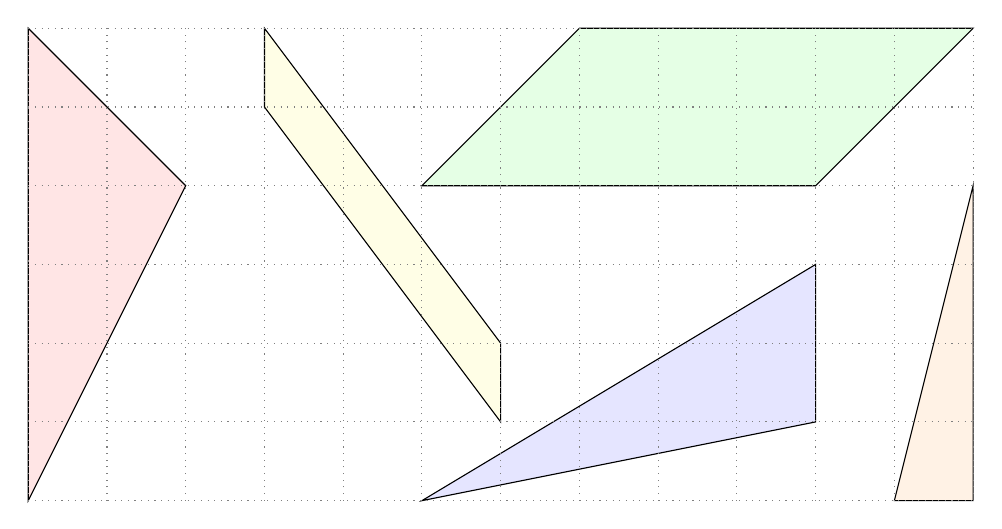
\begin{tikzpicture}
    \draw[fill=red!10] (0,6) -- (0,0) -- (2,4) -- cycle;
    \draw[fill=blue!10] (5,0) -- (10,1) -- (10,3) -- cycle;
    \draw[fill=yellow!10] (3,6) -- (3,5) -- (6,1) -- (6,2) -- cycle;
    \draw[fill=green!10] (7,6) -- (12,6) -- (10,4) -- (5,4) -- cycle;
    \draw[fill=orange!10] (12,4) -- (11,0) -- (12,0) -- cycle;
    \draw[color=gray, style=dotted] (0,0) grid[xstep=1cm, ystep=1cm] (12cm,6cm);
  \end{tikzpicture}

  Determine the areas of the indicated shapes.
\end{center}

\vgap

\begin{center}
  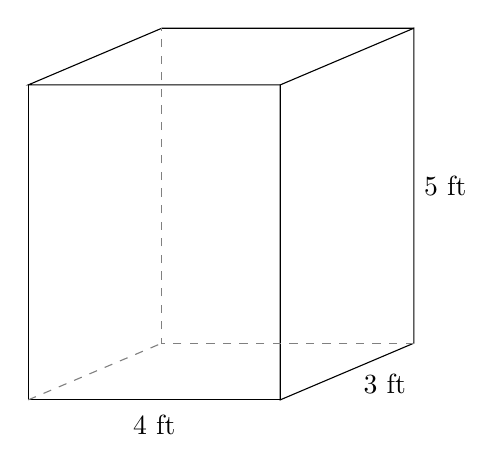
\begin{tikzpicture}[scale=.8, z={(-.707,-.3)}]
    \draw (4,0,0) -- (0,0,0) -- (0,5,0);
    \draw (4,0,0) -- (4,0,-3) -- (4,5,-3) -- (4,5,0) -- cycle;
    \draw (4,5,0) -- (0,5,0) -- (0,5,-3) -- (4,5,-3);
    \draw[style=dashed, color=gray] (4,0,-3) -- (0,0,-3) -- (0,5,-3);
    \draw[style=dashed, color=gray] (0,0,0) -- (0,0,-3); 
    \draw (2,-.4,0) node{4 ft};
    \draw (4.6,-.2,-1.5) node{3 ft};
    \draw (4.5,2.5,-3) node{5 ft};
  \end{tikzpicture}
  \hspace{5pc}
  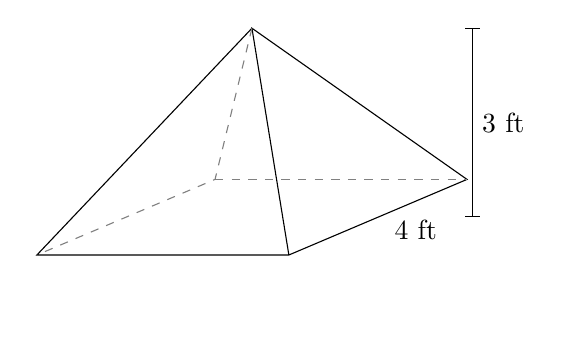
\begin{tikzpicture}[scale=.8, z={(.707,.3)}]
    \draw (2,3,2) -- (0,0,0) -- (4,0,0) -- (4,0,4) -- (2,3,2) --
    (4,0,0);
    \draw[color=gray, style=dashed] (2,3,2) -- (0,0,4) -- (0,0,0);
    \draw[color=gray, style=dashed] (0,0,4) -- (4,0,4);
    \draw (4.6,-.2,2) node{4 ft};
    \draw[|-|] (5.5,3,2) -- node[right] {3 ft} (5.5,0,2);

    % spacer
    \draw (0,-1,0) node {};
  \end{tikzpicture}

  Determine the length of the longest pole that can fit in the box, and
  determine the lengths of the edges of the pyramid.
\end{center}

\vgap

\begin{center}
  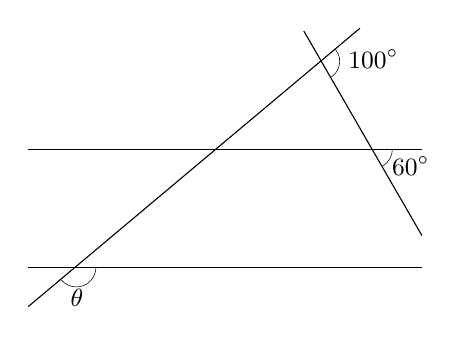
\begin{tikzpicture}
    %% background grid
    % \draw[color=gray, help lines, line width=.05pt] (-2,-2)
    % grid[xstep=.25cm, ystep=.25cm] (4,2);
    % \draw[color=black, help lines, line width=.1pt] (-2,-2)
    % grid[xstep=1cm, ystep=1cm] (4,2);
    % \draw[fill=red] (0,0) circle(.05);

    %% horizontal lines
    \draw (-2,-1) -- (3,-1);
    \draw (-2,.5) -- (3,.5);
    
    %% other lines
    \draw (-2,-1.5) -- ++(40:5.5);
    \draw (1.5,2) -- ++(-60:3);
    \draw[very thin] (2.625,.5) arc (0:-60:.25) node[right] {\small
      $60^\circ$};
    \draw[very thin] (1.9,1.77) arc (40:-60:.24) node[anchor=south west]
    {\small \ $100^\circ$};
    \draw[very thin] (-1.14,-1) arc (0:-140:.25) node[anchor=north west]
    {\small $\theta$};
  \end{tikzpicture}
  \hspace{2pc}
  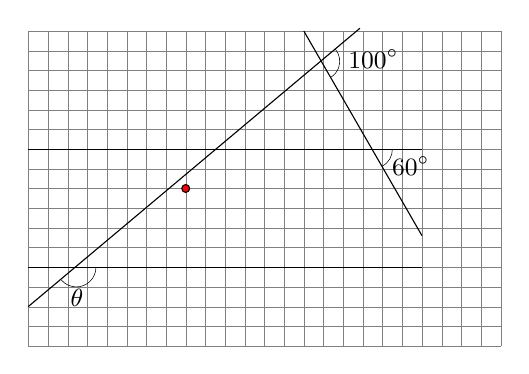
\begin{tikzpicture}
    %% background grid
    \draw[color=gray, help lines, line width=.05pt] (-2,-2)
    grid[xstep=.25cm, ystep=.25cm] (4,2);
    \draw[color=black, help lines, line width=.1pt] (-2,-2)
    grid[xstep=1cm, ystep=1cm] (4,2);
    \draw[fill=red] (0,0) circle(.05);

    %% horizontal lines
    \draw (-2,-1) -- (3,-1);
    \draw (-2,.5) -- (3,.5);
    
    %% other lines
    \draw (-2,-1.5) -- ++(40:5.5);
    \draw (1.5,2) -- ++(-60:3);
    \draw[very thin] (2.625,.5) arc (0:-60:.25) node[right] {\small
      $60^\circ$};
    \draw[very thin] (1.9,1.77) arc (40:-60:.24) node[anchor=south west]
    {\small \ $100^\circ$};
    \draw[very thin] (-1.14,-1) arc (0:-140:.25) node[anchor=north west]
    {\small $\theta$};
  \end{tikzpicture}

  Find the measure of the angle marked $\theta$.\\
  (Use the grid at right while drawing the diagram, to help determine where various things should be placed.)  
\end{center} 

\vgap

\begin{center}
  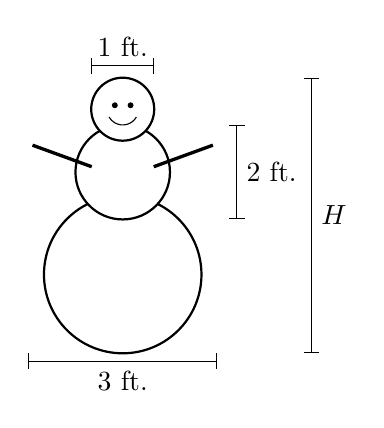
\begin{tikzpicture}
    \draw[thick, fill=white] (0,0) circle(1);
    \draw[thick, fill=white] (0,1.3) circle(.6);
    \draw[thick, fill=white] (0,2.1) circle(.4);
    \draw (0,2.1) ++(-30:.2) arc(-30:-150:.2);
    \draw[very thick] (0,1.3) ++(10:.4) --++(20:.8);
    \draw[very thick] (0,1.3) ++(170:.4) --++(160:.8);
    \draw[fill=black] (0,2.15) +(.1,0) circle(.03) +(-.1,0) circle(.03);
    \draw[|-|] (1.45,1.9) --node[right] {2 ft.} (1.45,.7);
    \draw[|-|] (-1.2,-1.1) --node[below] {3 ft.} (1.2,-1.1);
    \draw[|-|] (-.4,2.65) -- node[above] {1 ft.} (.4,2.65);
    \draw[|-|] (2.4,2.5) -- node[right] {$H$} (2.4,-1);
  \end{tikzpicture}
  \hspace{5pc}
  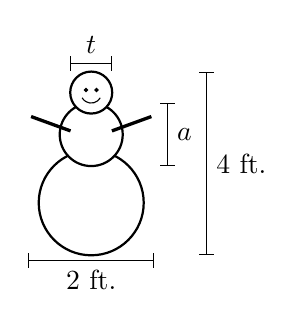
\begin{tikzpicture}[scale=2/3]
    \draw[thick, fill=white] (0,0) circle(1);
    \draw[thick, fill=white] (0,1.3) circle(.6);
    \draw[thick, fill=white] (0,2.1) circle(.4);
    \draw (0,2.1) ++(-30:.2) arc(-30:-150:.2);
    \draw[very thick] (0,1.3) ++(10:.4) --++(20:.8);
    \draw[very thick] (0,1.3) ++(170:.4) --++(160:.8);
    \draw[fill=black] (0,2.15) +(.1,0) circle(.03) +(-.1,0) circle(.03);
    \draw[|-|] (1.45,1.9) --node[right] {$a$} (1.45,.7);
    \draw[|-|] (-1.2,-1.1) --node[below] {2 ft.} (1.2,-1.1);
    \draw[|-|] (-.4,2.65) -- node[above] {$t$} (.4,2.65);
    \draw[|-|] (2.2,2.5) -- node[right] {4 ft.} (2.2,-1);
  \end{tikzpicture}

  Two similar snowmen.
\end{center}

\vgap

\begin{center}
  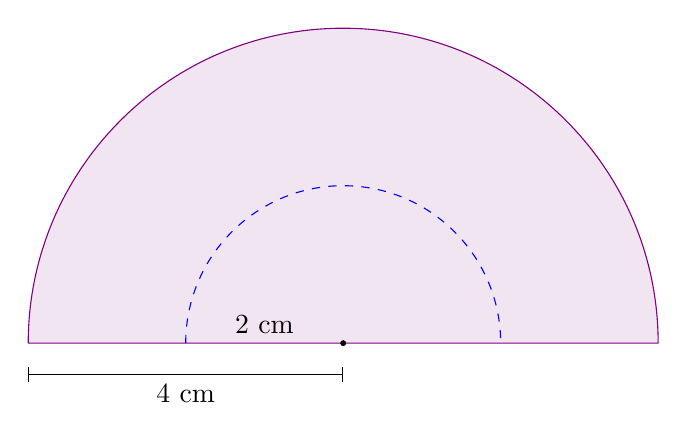
\begin{tikzpicture}[rotate=90]
    \draw[violet, fill=violet!10] (4,0) arc(90:-90:4) -- (4,-4) -- node[above, black]{$2$ cm} (4,-2)  -- (4,0);
    \draw[|-|]  (3.6,-4) -- node[below]{$4$ cm} (3.6,0);
    \draw[fill=black] (4,-4) circle(.03);
    \draw[blue, dashed] (4,-2) arc(90:-90:2);
  \end{tikzpicture}

  Pattern for a right circular cone.
\end{center}

\vgap

\newdimen\R
\R=1cm
\newdimen\S
\S=1.5cm
\begin{center}
  \begin{tikzpicture}
    % square
    \draw (0,0) -- (\S,0) -- (\S,\S) -- (0,\S) -- cycle;
    \draw (.5\S,-.5) node {\textbf{A}} 
    ++ (0,-.5) node {square};
    
    % pentagon
    \draw[xshift=3\R, yshift=.814\R] (90:\R) \foreach \x in {162,234,...,449} {
      -- (\x:\R)
    }-- cycle (0:\R);
    \draw[xshift=3\R] (0,-.5) node {\textbf{B}} 
    ++ (0,-.5) node {regular} ++ (0,-.5) node {pentagon};
    
    % parallelogram
    \draw[xshift=4.3\R] (0,0) -- (1.8\S,0) -- (2.3\S,.9\S) -- (.5\S,.9\S) -- cycle;
    \draw[xshift=4.3\R] (.9\S,-.5) node {\textbf{C}} 
    ++ (0,-.5) node {parallelogram};
    
    % octagon
    \draw[xshift=9.3\R, yshift=.925\R, rotate=22.5] (0:\R) \foreach \x in {45,90,...,359} {
      -- (\x:\R)
    } -- cycle (90:\R);
    \draw[xshift=9.3\R] (0,-.5) node {\textbf{D}} 
    ++ (0,-.5) node {regular octagon};
    
    % trapezoid
    \draw[xshift=10.5\R] (0,0) -- (2.8\S,0) -- node[rotate=-52]{$\vert$} (2\S,1.1\S) -- (.8\S,1.1\S)
    -- node[rotate=52]{$\vert$} (0,0);
    \draw[xshift=10.5\R] (1.4\S,-.5) node {\textbf{E}} 
    ++ (0,-.5) node {trapezoid};
  \end{tikzpicture}

  Some shapes.
\end{center}

\vgap

\begin{center}
  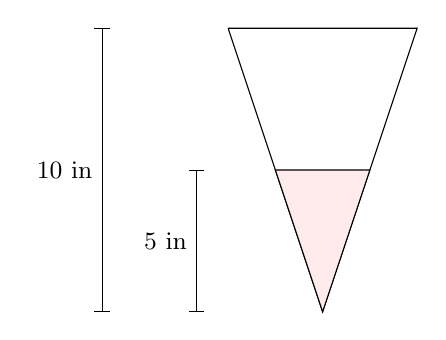
\begin{tikzpicture}[scale=.4]
    \draw[fill=none] (0,0) coordinate (o) 
    -- (3,-9) coordinate[pos=.5] (b)  coordinate (top)
    -- (6,0) coordinate[pos=.5] (a)
    -- (0,0);
    \draw[fill=red!08] (b) -- (a) -- (top) -- cycle;
    \draw[|-|] (-4,0) -- node[left] {\small 10 in} (-4,-9);
    \draw[|-|] (-1,-9/2) -- node[left] {\small 5 in} (-1,-9);
  \end{tikzpicture}
  \hspace{2pc}
  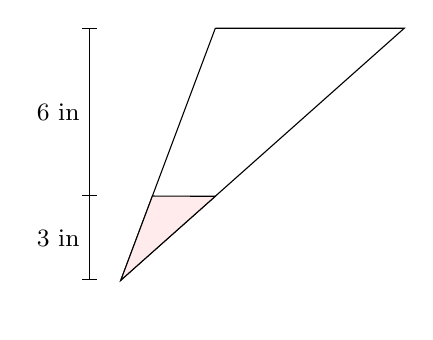
\begin{tikzpicture}[scale=.4]
    \draw[fill=none] (0,0) coordinate (o) 
    -- (-3,-8) coordinate[pos=.666] (b)  coordinate (top)
    -- (6,0) coordinate[pos=.333] (a)
    -- (0,0);
    \draw[fill=red!08] (b) -- (a) -- (top) -- cycle;
    \draw[|-|] (-4,0) -- node[left] {\small 6 in} (-4,-16/3);
    \draw[-|] (-4,-16/3) -- node[left] {\small 3 in} (-4,-8);
    \draw (0,-8.7) node {};
  \end{tikzpicture}

  Explain for each triangle what fraction of the total area is shaded.
\end{center}

\vgap

\begin{center}
  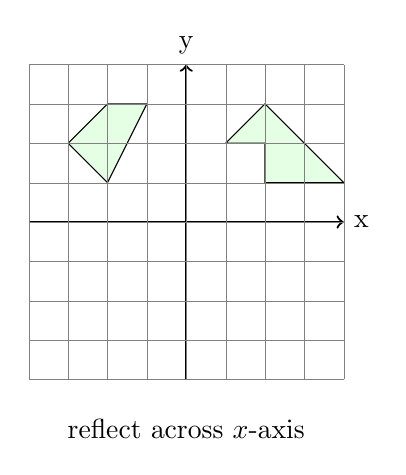
\begin{tikzpicture}[x=.5cm,y=.5cm]
    \draw[fill=green!10] (-1,3) -- (-2,3) -- (-3,2) -- (-2,1) -- cycle;
    \draw[fill=green!10] (2,3) -- (1,2) -- (2,2)-- (2,1) -- (4,1) --cycle;
    \draw[thick, ->] (0,-4) -- (0,4) node[above] {y};
    \draw[thick, ->] (-4,0) -- (4,0) node[right] {x};
    \draw[color=gray, help lines, line width=.05pt] (-4,-4)
    grid[xstep=.5cm, ystep=.5cm] (4,4);
    \draw (0,-4.75) node[below] {reflect across $x$-axis};
  \end{tikzpicture}
  \hspace{2pc}
  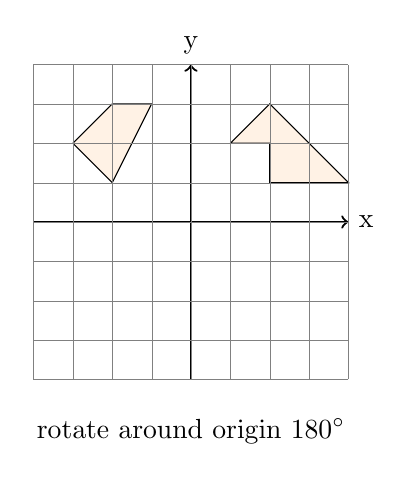
\begin{tikzpicture}[x=.5cm,y=.5cm]
    \draw[fill=orange!10] (-1,3) -- (-2,3) -- (-3,2) -- (-2,1) -- cycle;
    \draw[fill=orange!10] (2,3) -- (1,2) -- (2,2)-- (2,1) -- (4,1) --cycle;
    \draw[thick, ->] (0,-4) -- (0,4) node[above] {y};
    \draw[thick, ->] (-4,0) -- (4,0) node[right] {x};
    \draw[color=gray, help lines, line width=.05pt] (-4,-4)
    grid[xstep=.5cm, ystep=.5cm] (4,4);
    \draw (0,-4.75) node[below] {rotate around origin $180^\circ$};
  \end{tikzpicture}
  \hspace{2pc}
  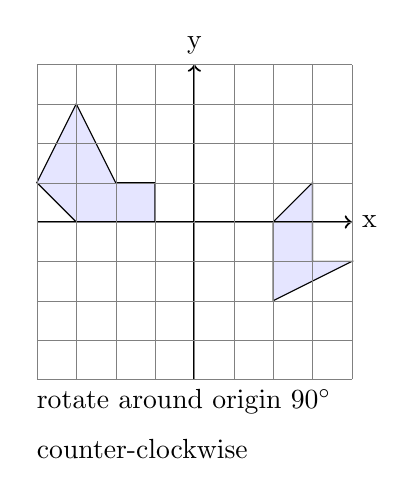
\begin{tikzpicture}[x=.5cm,y=.5cm]
    \draw[fill=blue!10] (-3,0) -- (-4,1) -- (-3,3) -- (-2,1) -- (-1,1)
    -- (-1,0) -- cycle;
    \draw[fill=blue!10] (3,1) -- (2,0) -- (2,-2) -- (4,-1) -- (3,-1) -- cycle;
    \draw[thick, ->] (0,-4) -- (0,4) node[above] {y};
    \draw[thick, ->] (-4,0) -- (4,0) node[right] {x};
    \draw[color=gray, help lines, line width=.05pt] (-4,-4)
    grid[xstep=.5cm, ystep=.5cm] (4,4);
    \draw (0,-4) node[below, text width=4cm] {rotate around origin $90^\circ$ counter-clockwise};
  \end{tikzpicture}

  Carry out the indicated transformations.  
\end{center}

\vgap

\begin{center}
  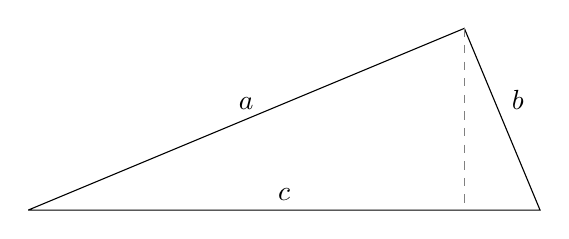
\begin{tikzpicture}[scale=.5]
    \draw (0,0) -- node[above]{$c$} (13,0) -- node[anchor=south west]{$b$} (144/13,60/13) coordinate
    (a) -- node[above]{$a$} (0,0);
    \draw[color=gray, line width=.5pt, dashed] (a) -- (144/13,0);
  \end{tikzpicture}
  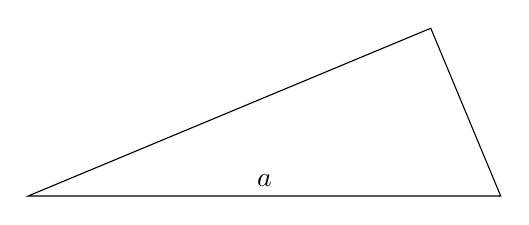
\begin{tikzpicture}[scale=.5*12/13]
    \draw (0,0) --  node[above] {$a$} (13,0) -- (144/13,60/13) -- cycle;
  \end{tikzpicture}
  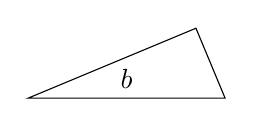
\begin{tikzpicture}[scale=.5*5/13]
    \draw (0,0) --  node[above] {$b$} (13,0) -- (144/13,60/13) -- cycle;
  \end{tikzpicture}

  Use these diagrams to give at least three different proofs of the Pythagorean theorem.  
\end{center}

\vgap

\begin{center}
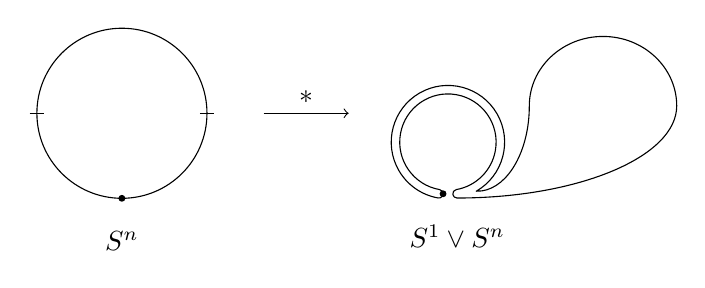
\begin{tikzpicture}[scale=1.8]
  \draw (-2.5,-.05) node (t) {} 
  arc(-90:0:.6cm) node (h1) {}
  arc(0:180:.6cm) node (h2) {}
  arc(180:270:.6cm);
  \draw[fill=black] (t) circle (.02);
  \draw[very thin] (h1) ++(-.05,0) -- ++(.1,0);
  \draw[very thin] (h2) ++(-.05,0) -- ++(.1,0);

  \draw (t) ++(0,-.3cm) node {$S^n$};

  \draw[->] (t) ++(1cm,.6cm) -- node[above]{$*$}++(.6cm,0);
  \draw[cap=round,join=round] (0,0) 
  arc(-60:260:.4cm) 
  arc(-100:0:.03cm)
  node(x){}
  arc(0:80:.03cm)
  arc(260:-80:.34cm)
  arc(100:270:.03cm)
  arc(-90:0:1.55cm and .65cm)
  arc(0:180:.52cm and .49cm)
  arc(0:-85:.367cm and .602cm)
  --cycle;

  \draw[fill=black] (x) circle(.02);
  \draw (x) ++(.1cm,-.3cm) node{$S^1 \vee S^n$};
\end{tikzpicture}

Map which gives the action of $\pi_1$ on $\pi_n$.
\end{center}

\vgap

\begin{center}
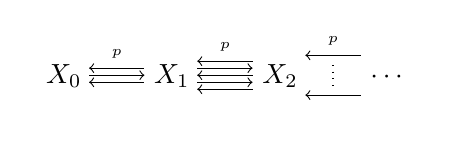
\begin{tikzpicture}
% requires the "matrix" library
\matrix (m) [matrix of math nodes, row sep=2em, column sep=1.7pc, text
width=1pc, text height=1pc, text depth=.5pc] { 
X_0  & X_1 & X_2 & \cdots \\
}; 

% decimals control start and end positions of arrows
\path[<-] 
(m-1-1.15) edge node[above] {\tiny $p$}  (m-1-2.165)
(m-1-1.-15) edge (m-1-2.-165);
\path[<-]
(m-1-2.28) edge node[above] {\tiny $p$} (m-1-3.152)
(m-1-2) edge (m-1-3)
(m-1-2.-28) edge (m-1-3.-152);
\path[<-]
(m-1-3.37) edge node (t) {} node[above] {\tiny $p$} (m-1-4.143)
(m-1-3.-37) edge node (b) {} (m-1-4.-143);

\path[->]
(m-1-1) edge (m-1-2);
\path[->]
(m-1-2.15) edge (m-1-3.165)
(m-1-2.-15) edge (m-1-3.-165);


\path[dotted]
(t) edge (b);
\end{tikzpicture}

A simplicial object.
\end{center}


\end{document}
